\documentclass[onecolumn]{IEEEtran}
\IEEEoverridecommandlockouts
% The preceding line is only needed to identify funding in the first footnote. If that is unneeded, please comment it out.
\usepackage{cite}
\usepackage{svg}
\usepackage{bookmark}
\usepackage{subfig}
\usepackage{amsmath,amssymb,amsfonts, amsthm}
\usepackage{lipsum}
\usepackage{placeins}
\usepackage{enumitem}
\usepackage{hyperref}
\usepackage{algorithmic}
\usepackage{tabularx}
\usepackage{graphicx}
\usepackage{textcomp}
\usepackage{xcolor}
\usepackage{tikz}
\def\BibTeX{{\rm B\kern-.05em{\sc i\kern-.025em b}\kern-.08em
    T\kern-.1667em\lower.7ex\hbox{E}\kern-.125emX}}
%
\newtheorem{theorem}{Theorem}[section]
\newtheorem{conjecture}[theorem]{Conjecture}
\newtheorem{proposition}[theorem]{Proposition}
\newtheorem{lemma}[theorem]{Lemma}
\newtheorem{claim}[theorem]{Claim}
\newtheorem{corollary}{Corollary}[theorem]
\newtheorem{definition}{Definition}[section]

\newcommand{\scn}[1]{\textnormal{\textsc{#1}}}
    
    
\begin{document}

\title{Counting Problem of \textit{PureCircuit}}

\author{\IEEEauthorblockN{Christos Demetriou}
\IEEEauthorblockA{\textit{Department of Computer Science} \\
\textit{University of Warwick}\\
Coventry, UK \\
u2018918@live.warwick.ac.uk, u2018918}}

\maketitle

\begin{abstract}
This project investigates the combinatorial structure of the \textsc{PureCircuit} problem.
We conjecture that its circuit-based formulation can provide insights and bounds on the counting complexity of \textsc{PPAD-1}.
In this report, we present the progress made so far, including preliminary results and ongoing developments.
In addition, we report on the construction of a visualisation tool designed to support the exploration and formulation of these combinatorial theorems.
Lastly we outline the current state of the project and explore the subsequent steps.

\end{abstract}

\begin{IEEEkeywords} % Index 
    Complexity Theory, Counting Complexity, Hazard Free Circuits, TFNP, PPAD, Search Problems, Kleene Logic
\end{IEEEkeywords}

\section{Introduction}
Over the last couple of years, there has been a revolutionary
initiative in the field of combinatronics.
Combinatronics has been a field of study in mathematics that primarily focused on
the notion of counting objects with certain properties. Over time, this notion
has shifted, especially in the subfield of algebraic combinatorics, where
there is no clear notion of the object that we are counting,
and the numbers express something more abstract \cite{pak_WhatCombinatorialInterpretation_2022}.
This gave a need to be able to assign a combinatorial interpretation to such numbers.
Being able to find such definitions or interpretations can be very important
as it allows us to utilise tools from combinatorics and allow us to understand
and reveal hidden structures and properties \cite{pak_WhatCombinatorialInterpretation_2022}. 
Moreover, there are several problems or numbers such as \textit{Kronecker coefficients} \cite{makar_AnalysisKroneckerProduct_1949},
whose combinatorial interpretation, would give a step towards the resolution of the $\textit{P} \neq \textit{NP}$
conjecture \cite{ikenmeyer_WhatWhatNot_2022, ikenmeyer_VanishingKroneckerCoefficients_2017}.


% To formalise that idea, Pak et al. has argued that if a function $f$
% belongs to $\textit{\#P}$, it implies that $f$ has a combinatorial interpretation
% \cite{pak_WhatCombinatorialInterpretation_2022, ikenmeyer_WhatWhatNot_2022}. We invest
In our current work, we focus on extending the work done by
Ikenmeyer et al., where they focused on the creation of frameworks
that determines whether $f \in^? \textbf{\#P}$, by looking
at the subclasses of $\textsc{\#TFNP}$ problems.
In our work we focus specifically on the $\textsc{PPAD}$ class of problems, under the lens of $\text{PureCircuit}$,
which utilises sequential Kleene-based circuits, to find satisfying assignments.
We hope to uncover many insights of the $\textsc{\#PureCircuit} -1$ problem 
as well as the limits of $\textsc{\#PPAD} -1$.

% In their paper, they were able to show that for a subclass of
% problems, also known as $\textit{PPAD} \subseteq \textit{TFNP}$,
% different $\textit{PPAD-complete}$ problems, may or may not have a combinatorial
% interpretation.


\subsection{Project objectives}

Below we will present our table of objectives. We will denote updated objectives with
(*), new objectives with (!), completed objectives with (\checkmark).

\begin{enumerate}[label*=R.\arabic*)]
    \item Find a parsimonious reduction from the $\textit{EndOfLine}$ to $\textit{PureCircuit}$.
    \item Improve the combinatorial bound between the reduction from EndOfLine to PureCircuit
    \item Demonstrate that $\textbf{\#}\text{PPAD}(PureCircuit)- 1 \not\subseteq \textbf{\#P}$
    \item Prove or disprove the following
\[
\forall n \in \mathbb{N}_{\geq 2} \exists c \in \mathbb{N}:  \scn{\#SourceOrExcess}(n, 1) \subseteq^c \scn{\#PureCircuit}
\]

\end{enumerate}

Below we will be representing the development portion of the project.

\begin{enumerate}[label=S.\arabic*)]
    \item Visualise and verify a \textsc{PureCircuit} instance.
    \item Generate a solution given a \textsc{PureCircuit} instance for a small number of nodes.
    \item Count the number of solutions of a  \textsc{PureCircuit} instance for a small number of nodes.
\end{enumerate}


We will compile the rest of the report, based on our current findings, how we modified our objectives to
the current ones as well as general reflections.


\subsection{Research Question}

Our main objectives revolve around the conjecture in \ref{conj:ppad-1-hardness}, where
we investigate the boundaries of $\scn{\#PPAD}-1$ with the help of the \textsc{PureCircuit} problem.
\begin{conjecturebox}{$\scn{\#PPAD}-1$ hardness}{ppad-1-hardness}
    Every lanaguage in \scn{PPAD} can be parsimoniously reduced up to some polynomial factor, to the
    pure circuit problem,  or more formally:
    $$
    \forall L \in \scn{PPAD}, \exists f \in n^{O(1)}: 
    \#L \subseteq^f \scn{\#PureCircuit}
    $$
\end{conjecturebox}

%
% Below we will present our main list of findings up to this point:
%
% \begin{theorem}[ND-Brouwer to PureCircuit]
%     Given $f(x) \triangleq 20$
%     $$
%     \scn{\#Brouwer}^{f_3} \subset^f \scn{\#PureCircuit}
%     $$
% \end{theorem}
%
% \begin{corollary}
%     For any $d \in \mathbb{N}_{\geq 2}$, we can define $f(\cdot) = \sum_{i = 1}^{d -1}  \binom{d}{i} 2^i$
%     such that:
%     $$
%     \scn{\#Brouwer}^{d} \subset^f \scn{\#PureCircuit}
%     $$ 
% \end{corollary}
%
%
%
% \begin{theorem}
%     For any $d \in \mathbb{N}_{\geq 2}$, we can define $f(\cdot) = 5$
%     such that:
%     $$
%     \scn{\#Brouwer}^d \subseteq^f \scn{\#PureCircuit}
%     $$ 
% \end{theorem}
%
%
% Throughout our search, we stumbled upon
% various variants of the problem as well as reductions and claims from other
% subclasses of PPAD or Hazard-Free logic
%
% \begin{proposition}
%     Weaker variants of PureCircuit can result to parsimonious reductions to the EndOfLine problem
%     as such:
%     \begin{gather*}
%         \scn{\#AcyclicBPureCircuit} \subseteq \scn{\#EndOfLine} \\
%         \scn{\#PermutationFreeBPureCircuit} \subseteq \scn{\#EndOfLine}
%     \end{gather*}
% \end{proposition}
%
%
% In addition, we were able to show that for different promise problems,
% we can find reductions to the PureCircuit problem
% %
% \begin{proposition}
%     $$
%         \scn{\#PUnsatHazard} \subseteq  \scn{\#PureCircuit}
%     $$
% \end{proposition}
%
% Lastly we introduce the following proposition
% \begin{proposition}
%     Given function $F: \mathbb{T}^n \to \mathbb{T}^n$
%     where $\mathbb{T} \triangleq \{0, 1, \bot\}$ and $F$ is a \textbf{natural}
%     function:
% $$
% \exists x^\star \in \mathbb{T}^n: F(x^\star) = x^\star
% $$
% \end{proposition}
% %
%
% The idea above is based on the Tarski Fixed point theorem.
% Using fixed points with the Kleene logic set, has been used in the past
% by Kozer as seen in his book \cite{kozen2006theory}, but we
% are extending such ideas to any possible functions or gates
% that use monotone gates. Doing that allows us to make the following observation.
%
% \begin{proposition}
%     $$
%     \scn{\#HazardTarski} \subseteq \scn{\#PureCircuit}
%     $$
% \end{proposition}
%


\section{Preliminaries and Background review}
% LTeX: enabled=true


\section{Current Progress}
\subsection{Theory Progress}
This section focuses on the theory progress we made.
We have experimented with various approaches
such as investigating easier variants of \textsc{PureCircuit} to find reductions
to the \textsc{EndOfLine}. Moreover, we looked into modifying the \textsc{Purify} gate
or finding a variant where we have more control over the $\bot$ value. We soon
realised that under Marino et al. \cite{marino_GeneralTheoryMetastable_1981} continuity
arguments, such variants are not guaranteed to exist.
Our core breakthrough was realised when experimenting with
Hazard-Free circuits  and \textit{UniqueEndOfPotentialLine}) problems. Specifically,
we looked at a problem by Fearnley et al. \cite{fearnley_UniqueEndPotential_2020} where
they introduced a variant Brouwer problems known as \textsc{OPDC}, which is a 
local descent problem with fixed point topologies. Combining ideas of the two 
lead to the main find of our project in \ref{sect:main-result}.


% In addition, for the last point, we made several efforts to ensure our problem is
% \textsc{PPAD}-complete and combinatorial friendly, by trying to restrict the \textsc{Purify} gate. 
% We soon realised that any methods that detect the $\bot$ value or try to eliminate ultimately
% fail. The observation can be based on a continuity argument that Marino created
% \cite{marino_GeneralTheoryMetastable_1981} and in general any possible extensions or gates we can
% add seem to adhere continuity. 




\subsubsection{$\scn{nD-StrongSperner}$ Constant Parsimonious Reduction} \label{sect:main-result}

% Daskalakis et al. \cite{daskalakis_ComplexityComputingNash_2006} showed that we can find a parsimonious reduction between
% $\scn{EndOfLine}$ and $\scn{3D-Brouwer}$, which is a variant of $\scn{3D-StrongSperner}$ and is based on the same principal. Later on
% Chen et al. \cite{chen_Complexity2DDiscrete_2009} was able to show that it suffices to use 
% 2 dimensions by reducing the problem to a 2D planar graph variant of \textsc{EndOfLine}.
The reduction from \textsc{StrongSperner} to \textsc{PureCircuit} was first
done by Deligkas et al. \cite{deligkas_PureCircuitTightInapproximability_2024},
under the condition of unbounded dimensionality and polynomial width and without any parsimonious bounds.
We offer a polynomial parimonious reduction \ref{def:func-pars}
for every $\scn{nD-StrongSperner}$ problem to  $\scn{PureCircuit}$.
We will subsequently demonstrate our reduction for 3 dimensions and then we will generalise.

\begin{theorembox}{3D-StrongSperner to PureCircuit}{thm:strong-pure}
    $$
    \scn{\#3D-StrongSperner} \subseteq^{7} \scn{\#PureCircuit}
    $$
\end{theorembox}

When referring to the fact that $x$ is a solution, we imply the definition described in  \ref{def:nd-strong-sperner}.
Additionally we will restrict the solution set of the \textit{Purify} gate of \textsc{PureCircuit}
to $(0,\bot),(\bot, 1), (0,1), (1, \bot)$. \ref{par:pure-circ-def} explains that this
does not affect the \textsc{PPAD-hardness} of the problem nor any counting arguments.
Lastly $\forall b \in \mathbb{B}^n, \bar{b}$ will denote the decimal representation of $b$.

\begin{proof} 
    Given input $(\lambda, 0^m)$, we first construct a colouring function $\Lambda: (\mathbb{B}^{(m+1)})^3$ such that:
$$
\forall (i,j,k) \in (\mathbb{B}^{(m+1)})^3: \Lambda(i,j,k) \triangleq 
\lambda\left( \left\lfloor  \frac{{\bar{i}+1}}{2}  \right\rfloor, \left\lfloor  \frac{{\bar{j}+1}}{2} \right\rfloor, \left\lfloor  \frac{{\bar{k}+1}}{2} \right\rfloor \right)  \\
$$

Conversely we can say that we map from our original domain to our new domain as such

\begin{equation}
    \label{eq:trans-eq}
    \forall  x \in (\mathbb{B}^{m})^3: \lambda(x) \to \{\Lambda[(\max\{2\bar{x_i} - b_i, 0\})_{i \in [3]}] \mid b \in \mathbb{B}^{3}\}
\end{equation}
The transformation can be visualised in the figure \ref{fig:main-proof:set_mapping}.
The reasoning for doubling the dimensions will be explained in the later sections.

\begin{figure}[h!]
    \centering
    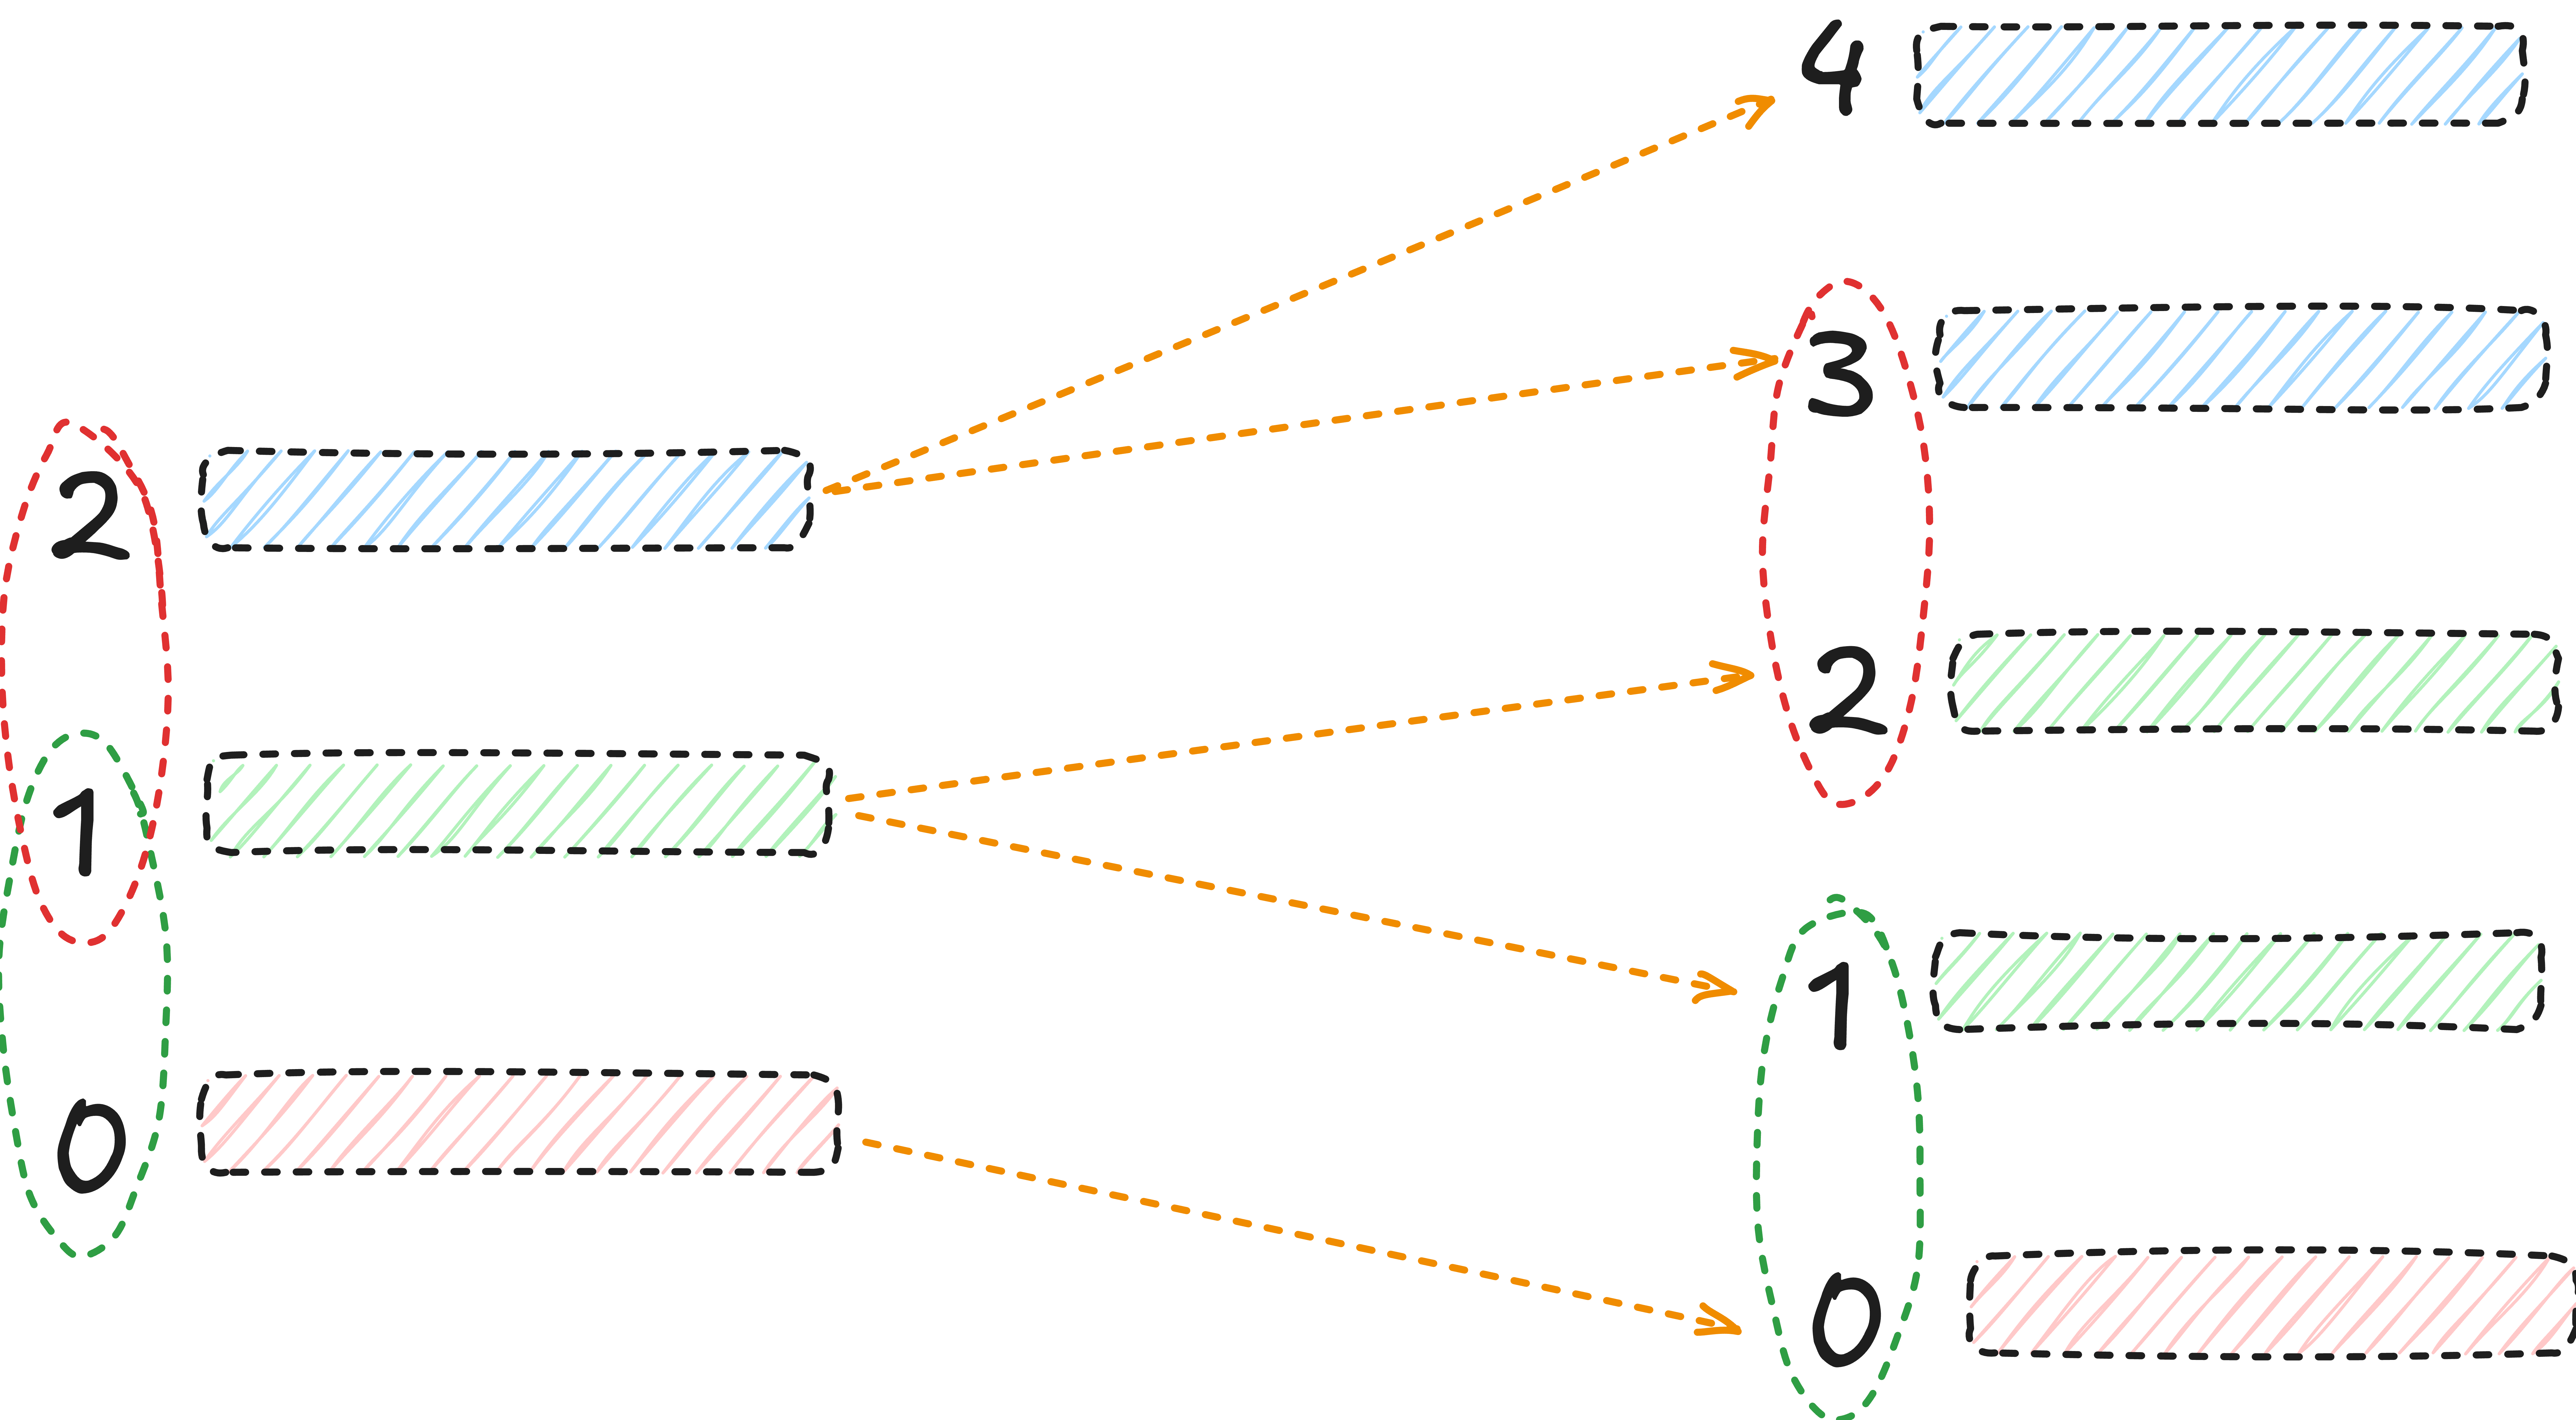
\includegraphics[width=0.5\textwidth]{assets/1751381227.png}
\caption{Transformation of solutions. In the original cube assume we have solutions $(0, i,j)$ and $(1, i,j)$ for some $i,j$. In our new mapping, these solutions correspond to
$(0, i,j), (2,i,j)$.}
    \label{fig:main-proof:set_mapping}
\end{figure}

Given that $S$ is the original set of solutions as described in \ref{def:nd-strong-sperner}, we define the claim \ref{clm:trans-main}.

\begin{claimbox}{Transformation claim}{trans-main}
    \label{clm:main-proof:trans-claim}
    Given $S_{\text{even}}$ the set of even solutions or more formally:
    $$
        S_{\text{even}} \triangleq
        \Big\{(i0,j0,k0) \in (\mathbb{B}^{(m+1)})^3 \mid (i0,j0,k0) \text{ covers all labels by \ref{def:bipolar-colouring}} \Big\}
    $$
    We claim $|S| = |S_{\text{even}}|$
\end{claimbox}

\begin{proof}
    We argue that we can bijectively map between $S \leftrightarrow S_{\text{even}}$.
    To show the left to right direction, assume $(i,j,k) \in S$.
    Using equation \ref{eq:trans-eq}, only the point $(2\bar{i}, 2\bar{j}, 2\bar{k}) = (i0, j0,k0)$ will be mapped to all even coordinates.
    Additonally, we can observe its neighbourhood set:
    $$
    N = \Big\{\Lambda(2\bar{i} + x_1, 2\bar{j} + x_2, 2\bar{k} + x_3) \mid x \in \mathbb{B}^3 \Big\}
    $$
    We can observe that WLOG $\Lambda(2i + 1, \cdot, \cdot) = \lambda(i + 1, \cdot, \cdot)$, which implies:
    $$
    N = \Big\{\lambda(\bar{i} + x_i, \bar{j} + x_j, \bar{k} + x_k) \mid x \in \mathbb{B}^3 \Big\}
    $$
    And therefore the point $(i0, j0,k0)$ is also a solution. We can use the previous neighbourhood argument to prove the converse direction.
\end{proof}
We will redefine $m + 1$ as $n$ to keep the notation consistent.
Given the above we provide a main sketch of our tranformation as such:
\begin{enumerate}
    \item \textbf{Input bits}: We initialize input nodes $s_1, s_2, s_3$
    \item \textbf{Bit generator}: We apply the \textit{Bit Generator gadget} $\hat{P}$ for each $s_i$,
        to create numbers $u^1, u^2, u^3 \in \mathbb{B}^{n}$.  We will use notation $\mathbf{x}[u^i]$ to
        describe the assingment of all nodes in $u^i$.
    \item \textbf{Circuit application}: We apply circuit $\bar{\Lambda}(u^1, u^2, u^3)$ to create output values $o_1, o_2, o_3$, where 
$\bar{\Lambda}$ is a 3-bit hazard-free variant of $\Lambda$.
    \item \textbf{Validation}: Copy the results to $s_1, s_2, s_3$
\end{enumerate}
The transformation can be summarised in the figure \ref{fig:main-proof:visualisation}.
The goal of the above transformation is to show that if $o_1 = o_2 =o_3 = \bot$, then we have a solution
to the original instance.

\begin{figure}[h!]
    \centering
    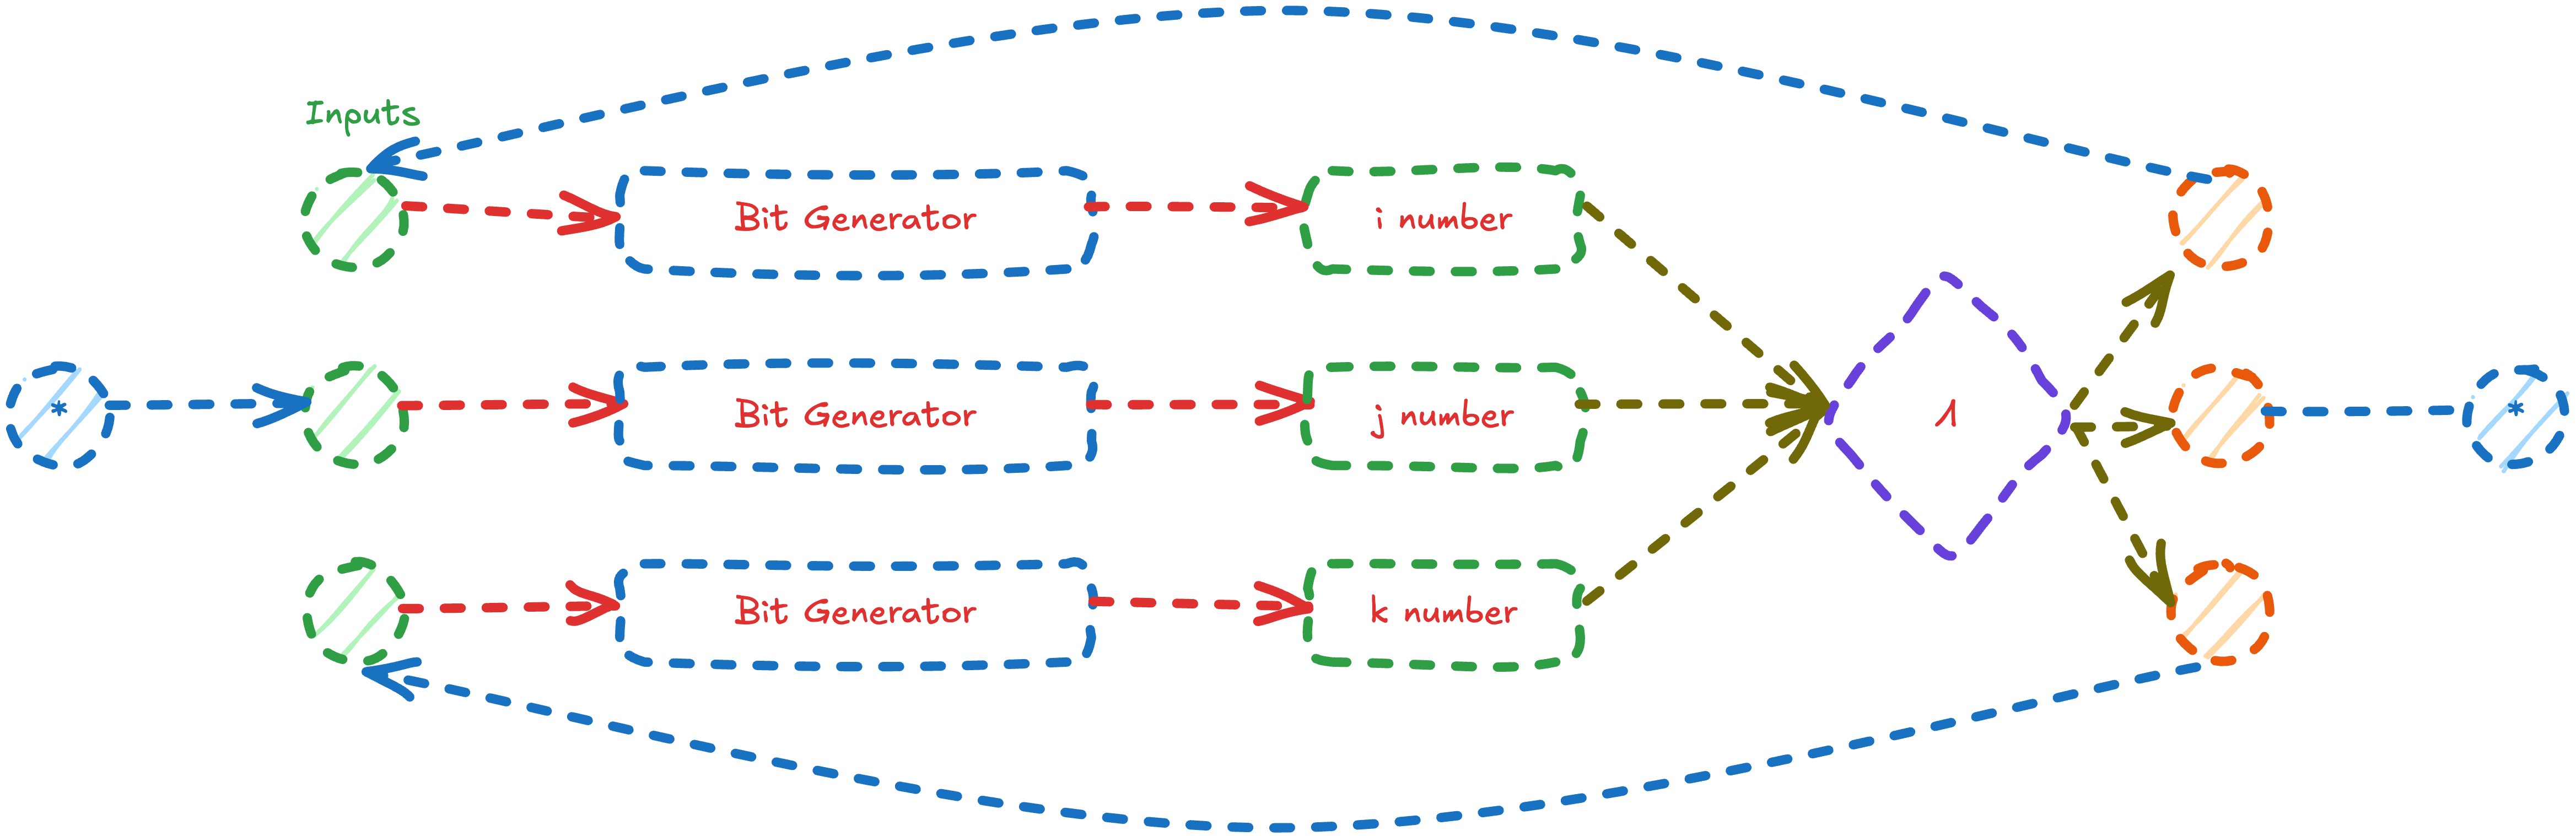
\includegraphics[width=0.75\textwidth]{assets/reduction_sketch.png}
    \caption{Construction map. The green nodes indicate the start nodes. The green squares indicate $u^1, u^2, u^3$. The orange circle denote
    $o_1, o_2, o_3$ and the blue lines denote the $\textit{COPY}$ operation to the starting nodes.}
    \label{fig:main-proof:visualisation}
\end{figure}


\paragraph{Bit generator}

We create the gadget described in the figure \ref{fig:main-proof:purification}.

\begin{figure}[h!]
    \centering
    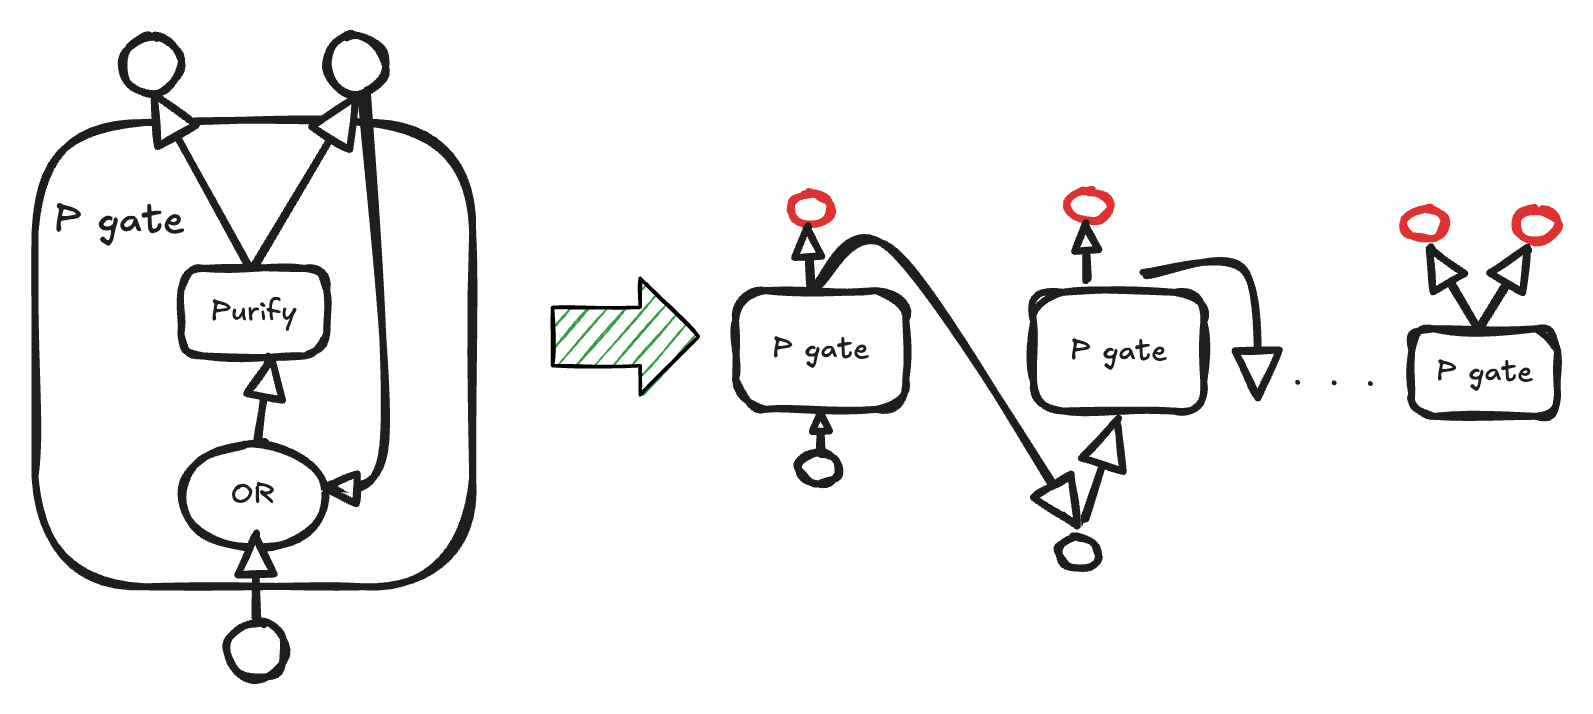
\includegraphics[width=0.5\textwidth, clip]{assets/purification_generator.png}
    \caption{Bit generator gadget which is defined as a linear stack of $P$ gates. The red nodes denote the output of the construction.} 
    \label{fig:main-proof:purification}
\end{figure}
\FloatBarrier

Given that construction we make the following lemma

\begin{lemma}[Bit Generator Lemma]
    \label{lem:bit-gen}
    The following hold true in our construction:
    \begin{enumerate}
        \item if $\mathbf{x}[s_i] = b \implies \mathbf{x}[u^i] = b^n$, given $b \in \mathbb{B}$
        \item if $\mathbf{x}[s_i] = \bot \implies \forall j \in [n-1]: \mathbf{x}[u^i_j] \in \mathbb{B}$ and $\mathbf{x}[u^i_{n}] \in \{1, \bot\}$
    \end{enumerate}
    The above translates to: if we have $\bot$ in our number, it can only be found in the LSB.
\end{lemma}

\begin{proof}
    The first part follows trivially from the defintion of the \textit{Purify} gate.
    To prove the second part of lemma, WLOG we choose $u^i$ out of the three outputs and
    assume $\exists j \in [n-1]: \mathbf{x}[u^i_j] = \bot$. It implies  that one of the purify gates had an output of $(\bot, 1)$.
    But due to our $\textsc{OR}$ gate, the input would be $1$ which implies the output is $1,1$, which leads to a contradiction.
\end{proof}


\paragraph{Circuit Application}

In the current phase, we apply a polynomial transformation to $\Lambda$ to be 3-bit hazard-free using the construction
by \textit{Corollary 1.10} \cite{ikenmeyer_ComplexityHazardfreeCircuits_2019} or 
by \textit{Corollary 1.9} \cite{bund_SmallHazardFreeTransducers_2025}.
By lemma \ref{lem:bit-gen}, we can have at most 3 $\bot$ values 
in our input. Using that property we create the lemma below:

\begin{lemmabox}{Circuit Application Lemma}{circuit}
    Given assignment $\mathbf{x}$ where $\mathbf{x}[o_1] = \mathbf{x}[o_2] = \mathbf{x}[o_3] = \bot$, it implies assingments of
    $\mathbf{x}[u^1], \mathbf{x}[u^2], \mathbf{x}[u^3]$
    correspond to a solution $(i0,j0,k0) \in S_\text{even}$
\end{lemmabox}


\begin{proof}
    First we argue that if $i\bot, j\bot, k\bot = \mathbf{x}[u^1],\mathbf{x}[u^2], \mathbf{x}[u^3]$, then
    its resolutions can represent hypercubes as shown in figure \ref{fig:main-proof:cube-vis}.
    \begin{figure}[h!]
        \centering
        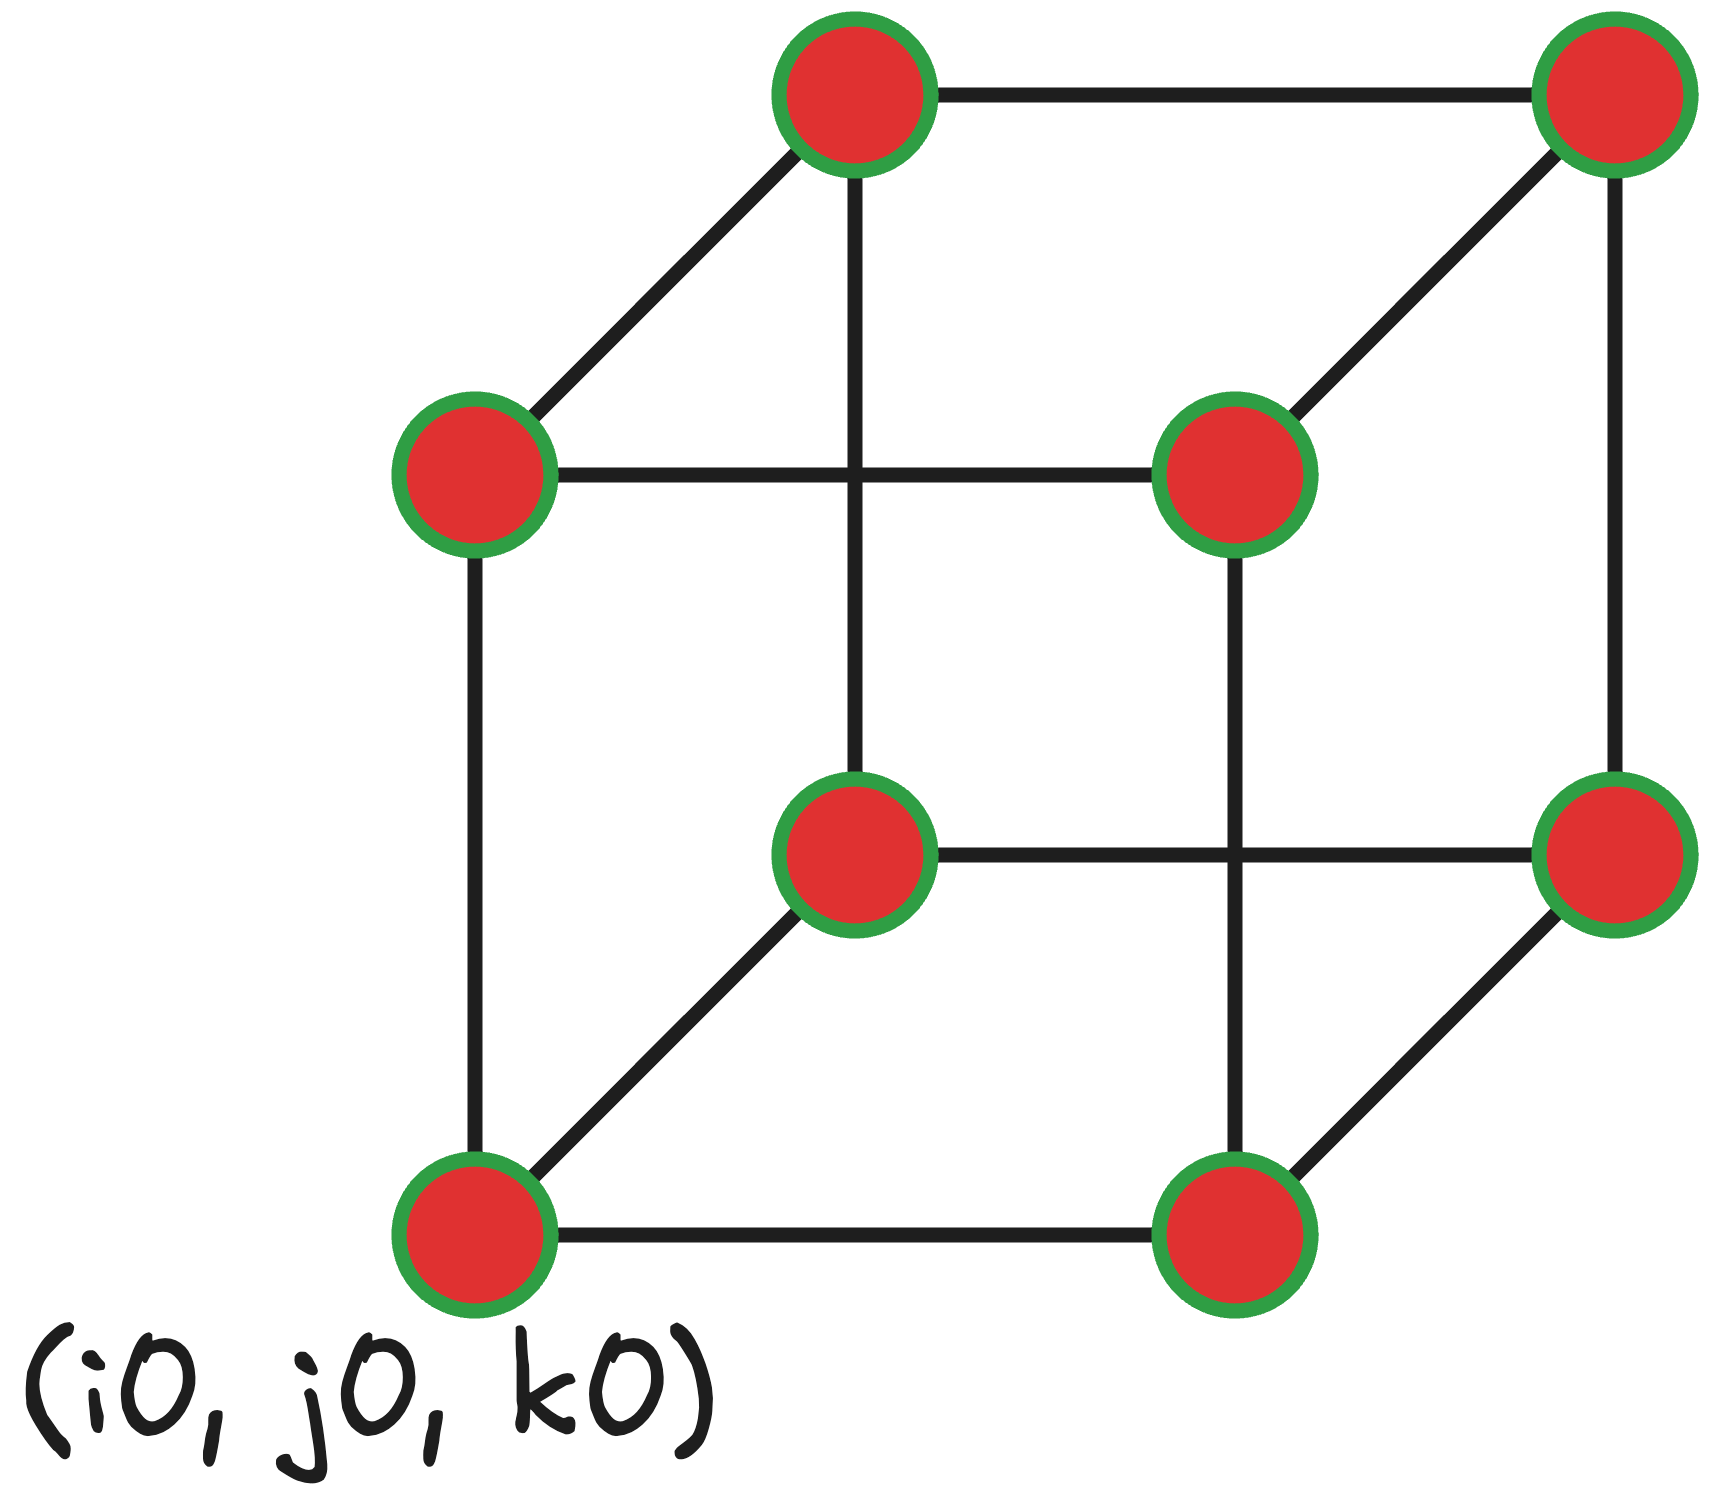
\includegraphics[width=0.2\textwidth]{assets/3d-cube.png}
        \caption{Resolutions of $i\bot, j\bot, k\bot$. We say the coordinate with the smallest $\|\cdot\|$ anchors the cube}\label{fig:main-proof:cube-vis}
    \end{figure}

    If $(i0, j0, k0)$ is a solution that implies:
    $$
    \forall i \in \{1,2,3\}, \exists c,c' \in \textsc{Res}(i\bot, j\bot, k\bot): [\bar{\Lambda}(c)]_i = +1 \wedge [\bar{\Lambda}(c')]_i = -1
    $$
    Since $\bar{\Lambda}$ is 3-bit hazard free, if all outputs are $\bot$, we satisfy the colouring criteria \ref{def:bipolar-colouring}.
\end{proof}
This also highlights the necessity of the initial domain transformation: 
it guarantees that all cube-aligned solutions are anchored at the $(i0, j0,k0)$ coordinates.
We can observe by fixing the LSB of the input to some value,
we extract a specific edge or face of the cube.


\begin{lemmabox}{Correctness lemma}{corr-lem}
    A valid assignment $\mathbf{x}$ of the current instance, corresponds to a point in $S_{\text{even}}$
\end{lemmabox}

\begin{proof}
    It suffices to show that a valid assignment only occurs when $\mathbf{x}[o_1] = \mathbf{x}[o_2] = \mathbf{x}[o_3] = \bot$. Assume
    $\exists i \in \{1,2,3\}$ such that label $i$ is not covered, meaning $\mathbf{x}[o_i] \neq \bot$.
    WLOG assume that $\mathbf{x}[o_i] = 0$. Our verification stage, will copy $0$ onto $s_i$. By lemma \ref{lem:bit-gen}, $\mathbf{x}[u^{(i)}] = 0^n$. From the boundary
    conditions of our circuits and the k-bit hazard-freeness construction,
    we know that $\Lambda(*, 0^n, *) = \{*, 1,  *\}$. But that implies
    $\mathbf{x}[o_i] = 1$ which leads to a contradiction. We can make a similar argument to when $\mathbf{x}[o_i] = 1$.
    Therefore, by \ref{lem:circuit}, if $\mathbf{x}[o_1] = \mathbf{x}[o_2] = \mathbf{x}[o_3]\bot$, we have a found a panchromatic
    solution of $S_\text{even}$.
\end{proof}

\end{proof}
\paragraph*{Counting Argument}
We observe that the LSB can only be $1,\bot$.
Moreover, we double count any edges or faces of the cube that cover all labels, which gives the equation:
$$
\underbrace{\binom{3}{1}}_{\substack{\text{One of the sides is odd} \\ \text{and covers all labels}}}
+ \underbrace{\binom{3}{2}}_{\substack{\text{One of the edges is odd} \\ \text{and covers all labels}}}
+ \underbrace{1}_{\text{All LSBs are } \bot} = 2^3 - 1 = 7
$$
Therefore, we can bound the number of solutions of \textsc{3D-StrongSperner} by a factor of $7$.


$\textsc{EndOfLine}$ problem parsimoniously reduces to $\textsc{2D-StrongSperner}$ and $\textsc{3D-StrongSperner}$
under \textbf{linear} colouring \cite{chen_Complexity2DDiscrete_2009, daskalakis_ComplexityComputingNash_2006}, but more
work has to been done in order to determine whether this still holds for bipolar colouring.


The reduction described above can work with any dimensionality
and $\forall n \in \mathbb{N}_{\geq 2}$, Chen et al. \cite{chen_SettlingComplexityComputing_2009} showed that
$\textsc{nD-StrongSperner}$ is still \textit{PPAD-Hard}.
Therefore the following corollary holds \ref{cor:pars-bounds}

\begin{corollarybox}{\scn{nD-StrongSperner} parsimonious reduction bounds}{pars-bounds}
    \begin{gather*}
        f(\cdot) = \sum_{i = 1}^{n}\binom{n}{i} = 2^n - 1 = a_n \\
        \scn{\#nD-StrongSperner} \subseteq^{a_n} \scn{\#PureCircuit}
    \end{gather*}
\end{corollarybox}


% Core breakthorugh came from the utilisation of the hazard-freeness from \cite{ikenmeyer_ComplexityHazardfreeCircuits_2019},
% as well as studying some problems in EOPL and UEOPL or more specifically the
% One-Permutation Discrete map. Athough in the end we were not able to extract any significantlly
% useful results out of it, its key observations were enough.

%
% \paragraph*{Useful Corollaries}

%
% To complete our last part of the theorem, it suffices to make use
% of the parsimonious reduction $\textsc{EndOfLine}$  to $\textsc{2D-StrongSperner}$ that Chen et al. \cite{chen_SettlingComplexityComputing_2009}.
% It has to be denoted that a similar reduction was made by
% Daskalakis et al. \cite{daskalakis_ComplexityComputingNash_2006}, where
% he reduced $\textsc{EndOfLine}$ to $\textsc{3D-StrongSperner}$ parsimoniously
% with similar ideas.
% For our theorem we will refer to the $\textsc{2D-StrongSperner}$ reduction and
% conclude with the theorem.
%
%
% \begin{theorem}[From $\scn{EndOfLine}$ to $\scn{PureCircuit}$]
% $$
% \scn{\#EndOfLine} -1 \subseteq \scn{\#2D-StrongSperner} -1 \subseteq^5 \scn{\#PureCircuit} -1
% $$
% \end{theorem}
%
% \subsubsection{Hazard-Free Logic Findings}
%
% Whilst trying to tackle the main objectives of the dissertation, we stumbled upon
% several interest relations across Hazard. We will use the notion of
% promise problems to show the following relation. First we will
% define a variant of UnSAT hazard as explained in \cite{ikenmeyer_ComplexityHazardfreeCircuits_2019}.
%
% \begin{definition}
%     Given a circuit $C$ that computes $f : \mathbb{B}^n \to \mathbb{B}$ such that
%     $\forall x \in \mathbb{B}^n : f(x) = 0$, find $\bar{x} \in \mathbb{T}^n$ such that
%     $C(\bar{x}) = \bot$. We assume that $\forall x \in \mathbb{B}^n: C(x) = 0$.
% \end{definition}
%
% Given the idea above we propose the following:
%
% \begin{proposition}
%     $$
%         \scn{\#PromiseUnsatHazard} \subseteq  \scn{\#PureCircuit} -1
%     $$
% \end{proposition}
%
% For the purposes of the current reduction, we will use the same \textsc{Purify} values
% $(0,1), (0,\bot), (1,\bot), (\bot, 1)$
%
% \paragraph{Construction}
% We start with a single node $s$. We create $n$ copies of \textsc{Purify}, where all 
% use $s$ as the input. From each purify gate we use the left output and
% create a vector $\hat{x} \in \mathbb{T}^n$ and pass them
% onto $C$ which will output onto a node $o$. We copy the output onto $s$.
% The above description can be summarised in the following figure \ref{fig:unsat-proof}.
%
% \begin{figure}[h!]
%     \centering
%         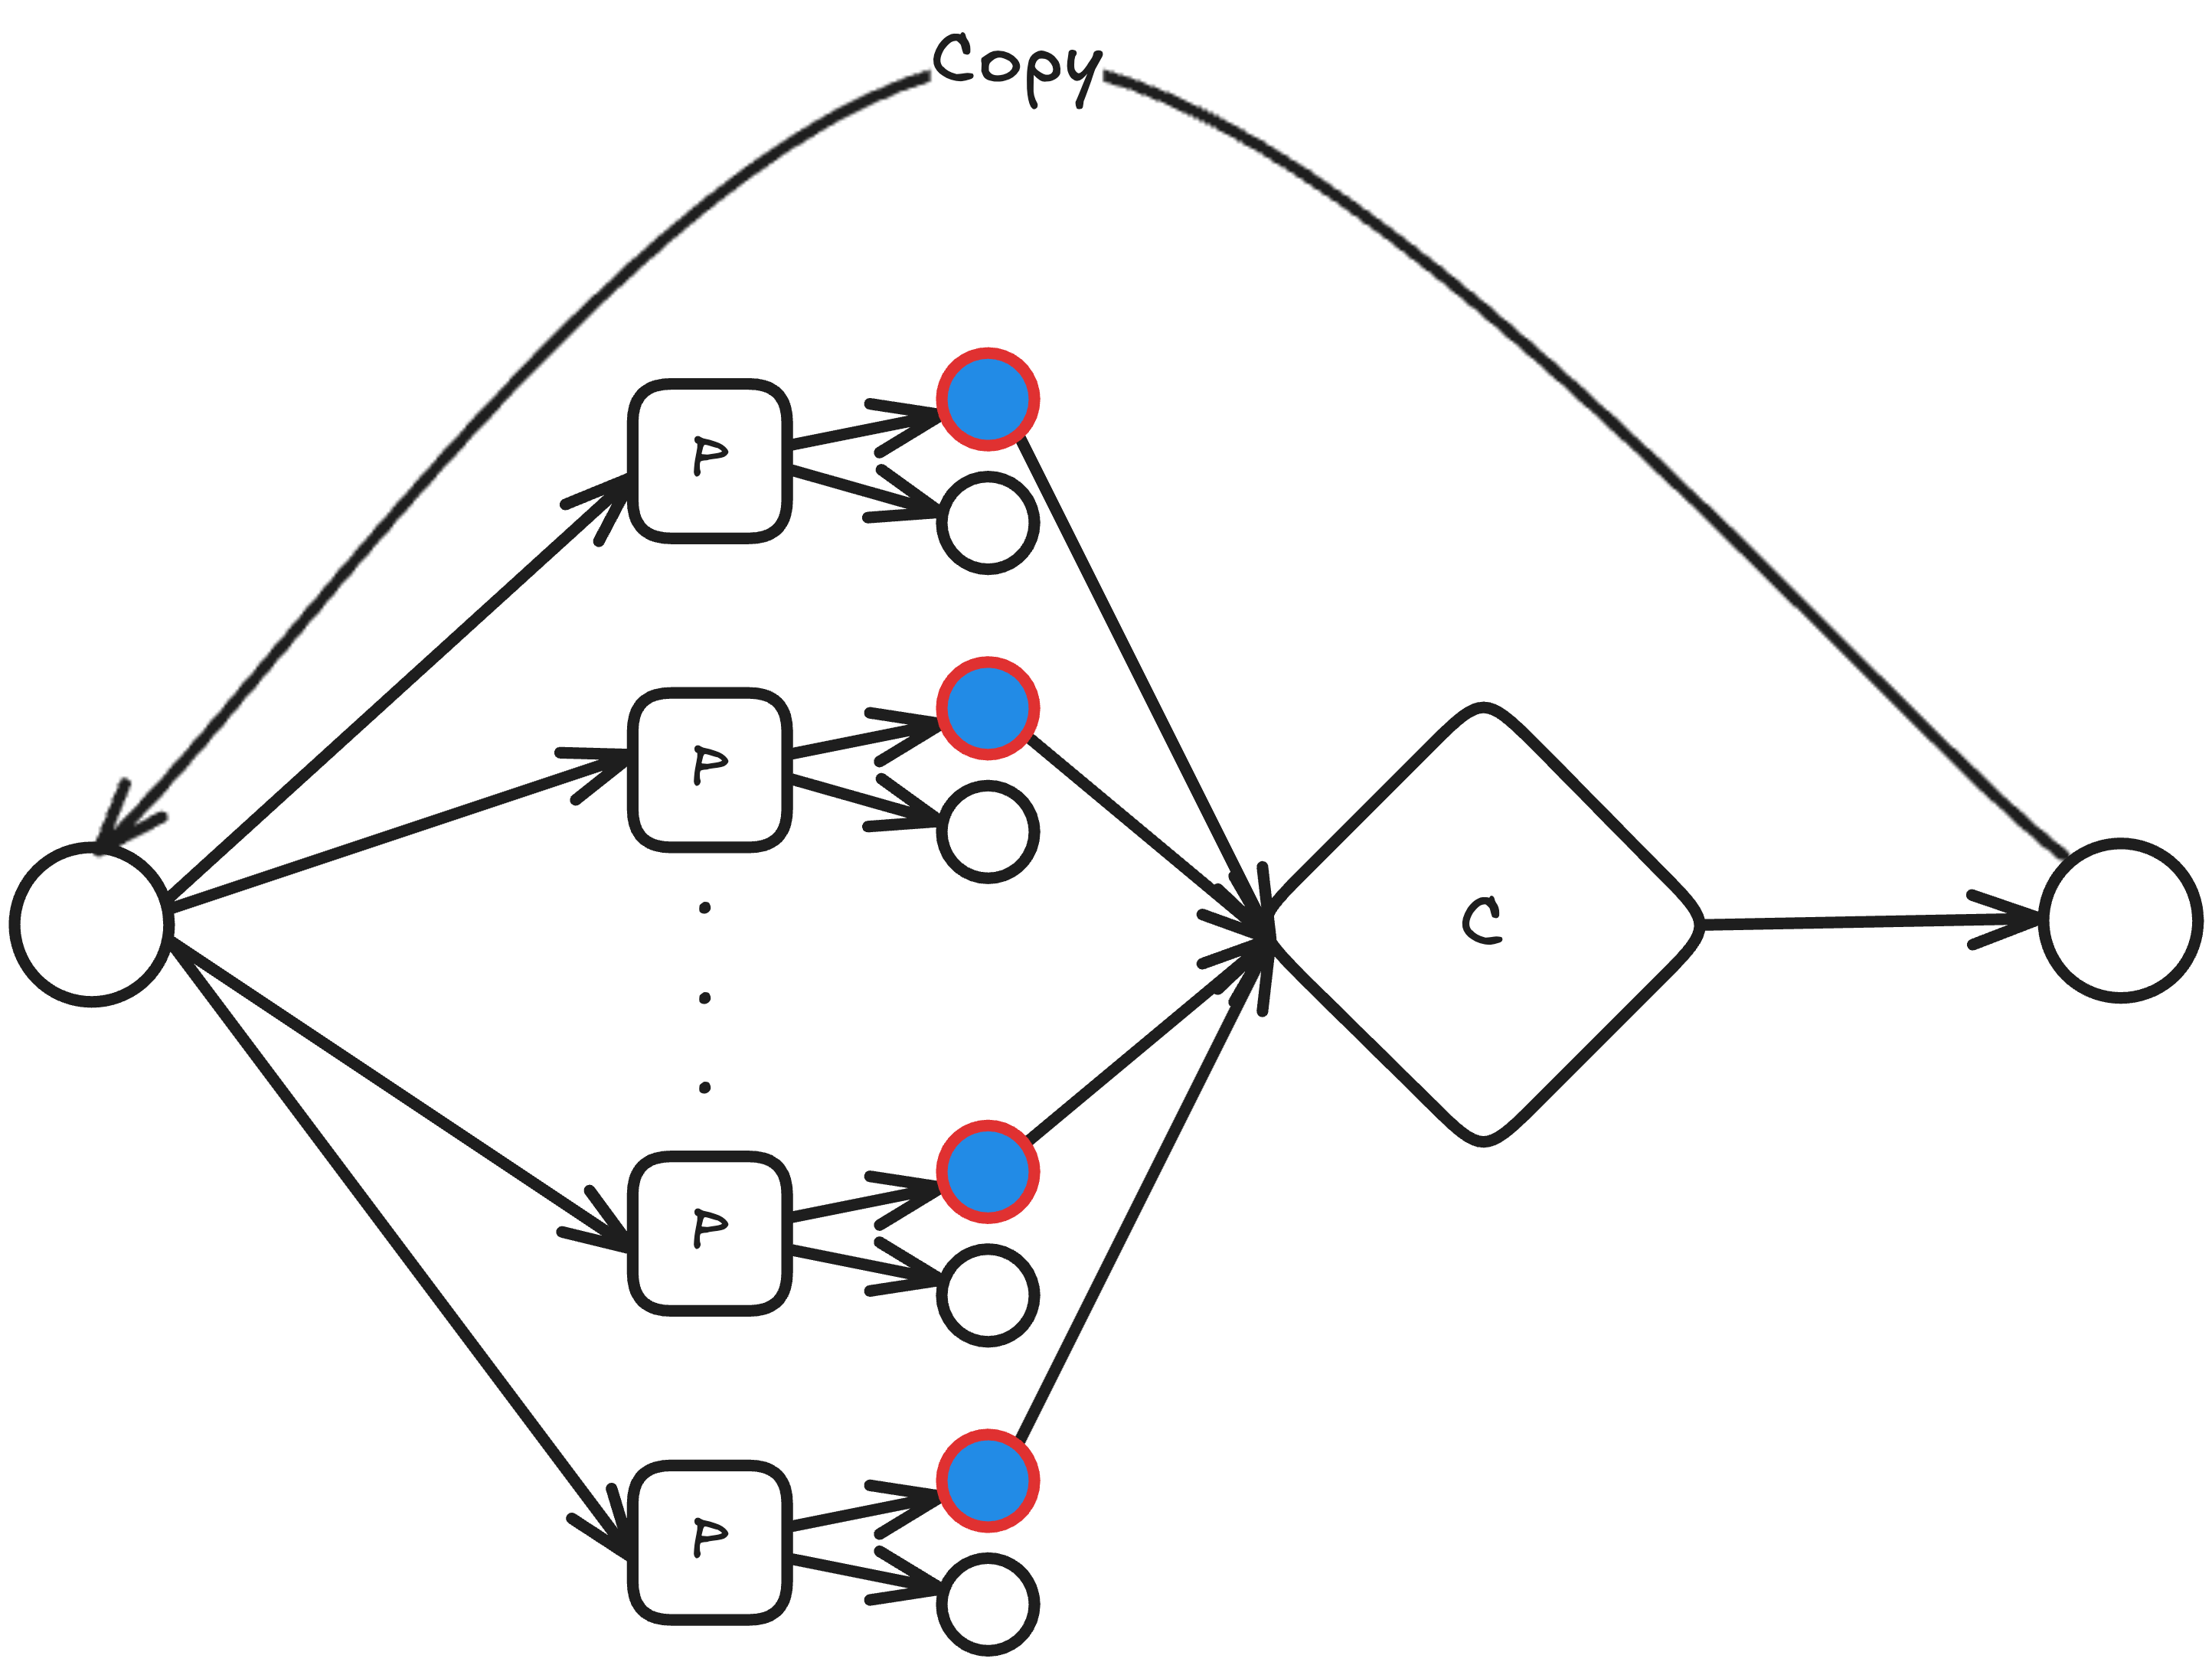
\includegraphics[width=0.5\textwidth]{assets/circuit-unsat.png}
%     \caption{Pure Circuit construction}
%     \label{fig:unsat-proof}
% \end{figure}
%
% \begin{proof}
% To prove our counting argument, we can make the following observation:
% If $o = 0$, we are computing $C(0^n) = 0$, which is the one guaranteed solution.
% We know that $o \neq 1$, therefore the only other possible solutions are $\bar{x} \in \mathbb{T}^n: C(\bar{x}) = \bot$.
% We also know from our construction of our \textsc{Purify} gate values, that our highlighted nodes
%     can take values $\{0,1,\bot\}$. Therefore, given that $\hat{x} \in \mathbb{T}^n$,
% our construction can find all possible solutions.
% \end{proof}
%

\subsubsection{Hazard Circuits and Tarski}
We define the following subclass of \textsc{Tarski} \ref{def:tarski-ppad}:


\begin{definitionbox}{$\scn{KleeneTarski}$ problem definition}{kleene-tarski}
    Given $F: \mathbb{T}^n \to \mathbb{T}^n$, where $F$ is a \textit{natural} function \ref{def:nat-func},
    find $x \in \mathbb{T}^n$ such that $F(x) = x$
    We assume $F$ will be represented as a circuit that uses set of gates
    $\{\wedge, \vee, \neg, \mathbf{0}, \mathbf{1}\}$.
\end{definitionbox}

\begin{proposition}[Parsimonious Reduction between $\scn{KleeneTarski}$ and $\scn{PureCircuit}$]
    $$
    \scn{\#KleeneTarski} \subseteq \scn{\#PureCircuit}
    $$
\end{proposition}

\begin{proof}
    Given an input circuit $C: \mathbb{T}^n \to \mathbb{T}^n$, construct $\textsc{PureCircuit}$ instance:
\begin{enumerate}
    \item Initiate a vector of $n$ nodes, which we denote as $s$.
    \item Construct the $C$ using the standard set of gates and apply $C(x)$ to create output vector $o$.
    \item Copy the results back into $s$.
\end{enumerate}

\begin{figure}[h!]
    \centering
    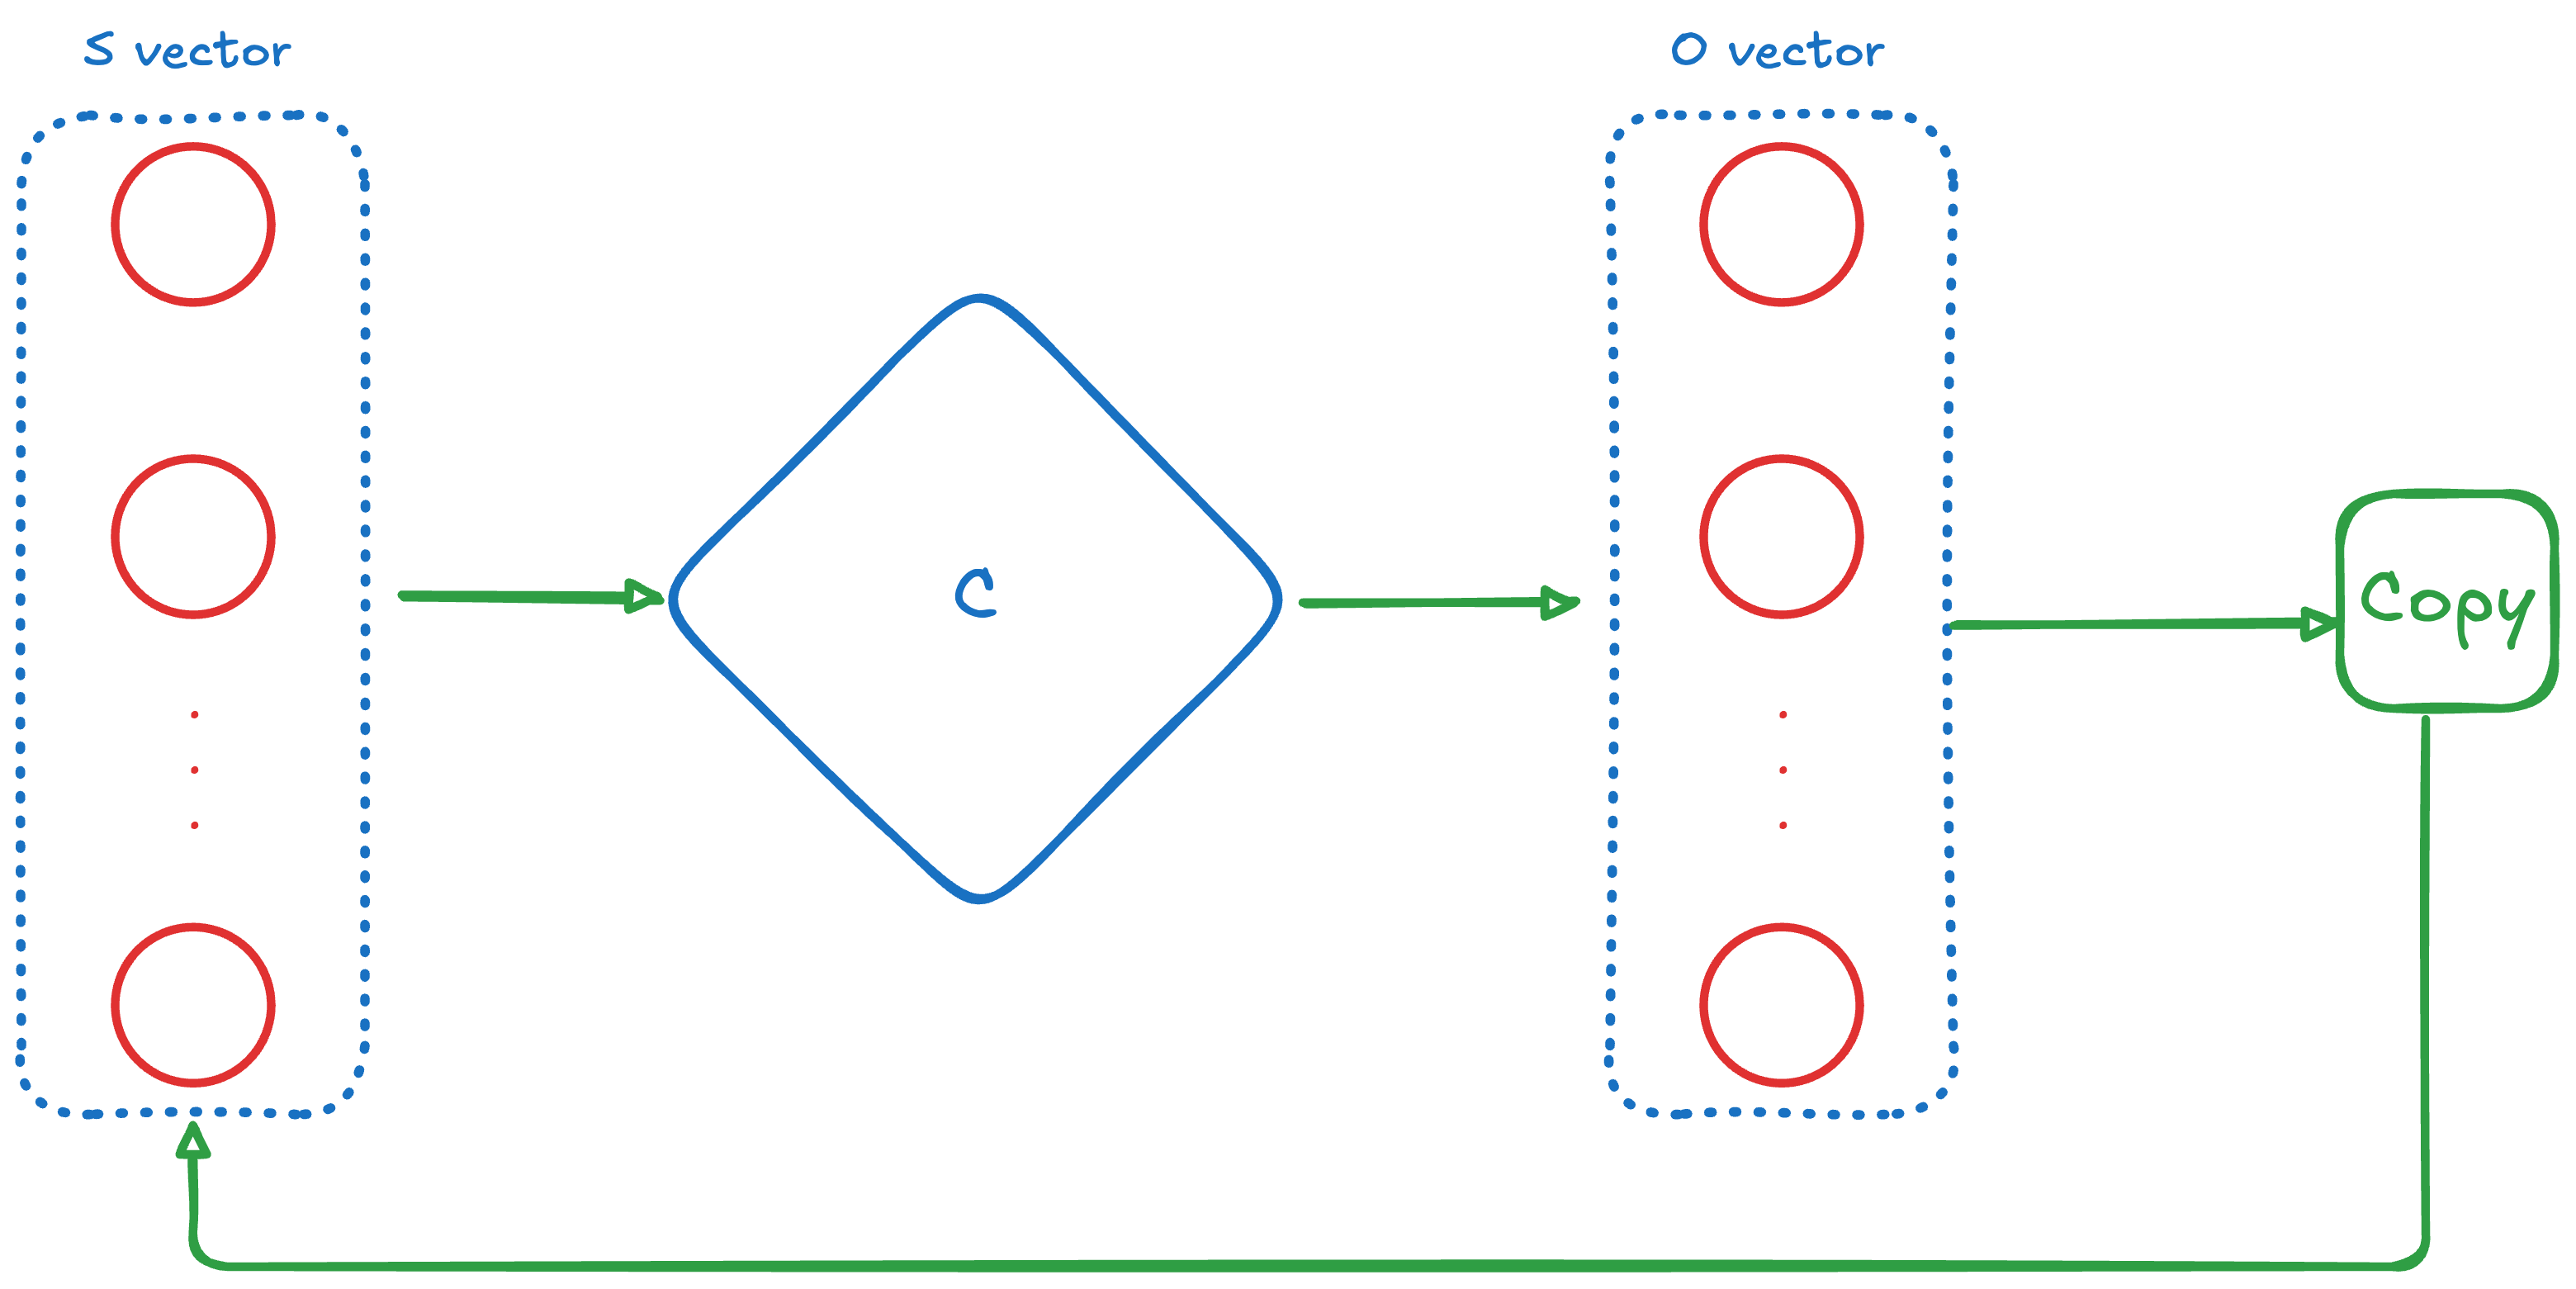
\includegraphics[width=0.5\textwidth]{assets/tarski-constrution.png}
    \caption{\textsc{Tarski} construction}\label{fig:tarski-constr}
\end{figure}


We can visualise the above construction in figure \ref{fig:tarski-constr}.
We can observe that, for any valid assignment $\mathbf{x} \implies \mathbf{x}[s]= \mathbf{x}[o]$,
which implies $\mathbf{x}[o] = F(x) = \mathbf{x}[s]$.
\end{proof}



% \subsubsection{Reductions to the EndOfLine}
%
% One can also attempt to make some reductions to the \textsc{EndOfLine}. It has to be noted,
% that we assume that there are no parsimonious reductions to the \textsc{EndOfLine},
% but we were able to construct some variants that allows to make there reductions.
% They key insights for this comes from the \textsc{PPAD}-inclusion proof
% by Deligkas et al. \cite{deligkas_PureCircuitTightInapproximability_2024}, where they
% showed that we can reduce PureCircuit, to \textit{Brouwer} problem by constructing
% a continuous function $F: [0,1]^n \to [0,1]^n$ as such: For each $v \in V$, we create
% continuous functions $f_i(\cdot): [0,1]^n \to [0,1]$ where we take thne input of vector
% of all the nodes and output the value of the current node
% \begin{enumerate}
%     \item If $v \in V$ is the output of a $\textsc{NOR}$ gate with inputs $x_1, x_2$, then we have:
%         $$
%         f_v(\mathbf{x}) := (1 - \mathbf{x}_{x_1}) \cdot (1 - \mathbf{x}_{x_2})
%         $$
%     \item If $y_1, y_2$ are the outputs of a  $\textsc{Purify}$ gate with $z$ as input, then we have:
%         \begin{align*}
%             f_{y_1}(\mathbf{x}) &:= \max\{2 \cdot \mathbf{x}_{z} - 1, 0\}\\
%             f_{y_2}(\mathbf{x}) &:= \min\{2 \cdot \mathbf{x}_{z}, 1\}
%         \end{align*}
% \end{enumerate}
% If $F(x) = x$, then we also found a solution for \textsc{PureCircuit} by:
% $$
% \forall v \in V: \mathbf{x}[v] = \begin{cases}
%     0 & \mathbf{x}[v] = 0 \\
%     \bot & 0 < \mathbf{x}[v] < 1 \\
%     1 & \mathbf{x}[v] = 1 \\
% \end{cases}
% $$
% Given that as an assumption we can restrict our \textit{Purify} gate
% to outputs $(0,\bot), (0,1), (\bot, 1)$. Using that we can define two types of variants
% of \textsc{PureCircuit} that are parsimoniously reducible to \textsc{SourceOrPresink}.
% We first define \textsc{SourceOrPresink} as:
%
% \begin{definition}[$\scn{SourceOrPresink}$ definition]
%     A $\scn{SourceOrPresink}$ is defined by the same construction as the $\scn{EndOfLine}$ 
%     but the solutions are sources and predecessors of sinks. If a node is both a source
%     and a presink, then we count it once.
% \end{definition}
%
% We will annotate our \textit{Purify} gates with an additional bit $b \in \mathbb{B}$ such that
% $$
% \forall x \in \mathbb{T}, y_1, y_2 \in \mathbb{T}: \textsc{Purify}^b(x) = (y_1,y_2) \implies \textsc{Purify}^{\neg {b}}(x) = (y_2, y_1)
% $$
% We can create two types of problems based on the annotation:
% \begin{enumerate}
%     \item Acyclic \textsc{PureCircuit}: Our instance is acyclic
%     \item Permutation-free \textsc{PureCircuit}: The outputs of a pure circuit, are connected to a circuit such that any permutation of the inputs
%         retains the result. More formally:
%         $$
%         \forall x \in \mathbb{T}^n, \sigma \in \mathcal{A}: C(\sigma(x)) = C(x)
%         $$
%         Where $\mathcal{A}$ is the set of automorphisms of $[n] \to [n]$.
%         The above description can be depicted in the following figure:
%         (ADD FIGURE)
% \end{enumerate}
%
% We can show that above variants we can create the following proposition (ref).
% To prove the reduction we can need to argue that we can go from one solution to another.
% The core idea of these problems is:  if we find a solution given in 
% a set of configurations $\gamma \in \{0,1\}^p$ where $p$ are the number of purify gates,
% we can match it with an additional solution where our set of configurations is $\neg \gamma$.
% This can be visualised as such: If the flip does not affect the inputs then we
% can create the following graph:
%
% \begin{figure}[h!]
% \centering
%
%
% \tikzset{every picture/.style={line width=0.75pt}} %set default line width to 0.75pt        
%
% \begin{tikzpicture}[x=0.75pt,y=0.75pt,yscale=-1,xscale=1]
% %uncomment if require: \path (0,260); %set diagram left start at 0, and has height of 260
%
% %Shape: Circle [id:dp7760056968770814] 
% \draw   (90,140) .. controls (90,123.43) and (103.43,110) .. (120,110) .. controls (136.57,110) and (150,123.43) .. (150,140) .. controls (150,156.57) and (136.57,170) .. (120,170) .. controls (103.43,170) and (90,156.57) .. (90,140) -- cycle ;
%
% %Shape: Circle [id:dp22383258291194785] 
% \draw   (190,140) .. controls (190,123.43) and (203.43,110) .. (220,110) .. controls (236.57,110) and (250,123.43) .. (250,140) .. controls (250,156.57) and (236.57,170) .. (220,170) .. controls (203.43,170) and (190,156.57) .. (190,140) -- cycle ;
%
% %Straight Lines [id:da1444295916995948] 
% \draw    (150,140) -- (188,140) ;
% \draw [shift={(190,140)}, rotate = 180] [color={rgb, 255:red, 0; green, 0; blue, 0 }  ][line width=0.75]    (10.93,-3.29) .. controls (6.95,-1.4) and (3.31,-0.3) .. (0,0) .. controls (3.31,0.3) and (6.95,1.4) .. (10.93,3.29)   ;
%
% % Text Node
% \draw (120,140) node   [align=left] {A};
% % Text Node
% \draw (220,140) node   [align=left] {B,C};
%
%
% \end{tikzpicture}
% \caption{Equal solution conversion}
% \label{fig:equal}
% \end{figure}
% Otherwise for two distinct solutions we can use the following
% \begin{figure}[h!]
% \centering
% \tikzset{every picture/.style={line width=0.75pt}} %set default line width to 0.75pt
% \begin{tikzpicture}[x=0.75pt,y=0.75pt,yscale=-1,xscale=1]
% %uncomment if require: \path (0,260); %set diagram left start at 0, and has height of 260
%
% %Shape: Circle [id:dp7760056968770814] 
% \draw   (90,140) .. controls (90,123.43) and (103.43,110) .. (120,110) .. controls (136.57,110) and (150,123.43) .. (150,140) .. controls (150,156.57) and (136.57,170) .. (120,170) .. controls (103.43,170) and (90,156.57) .. (90,140) -- cycle ;
%
% %Shape: Circle [id:dp22383258291194785] 
% \draw   (190,140) .. controls (190,123.43) and (203.43,110) .. (220,110) .. controls (236.57,110) and (250,123.43) .. (250,140) .. controls (250,156.57) and (236.57,170) .. (220,170) .. controls (203.43,170) and (190,156.57) .. (190,140) -- cycle ;
%
% %Shape: Circle [id:dp48038379742035975] 
% \draw   (290,140) .. controls (290,123.43) and (303.43,110) .. (320,110) .. controls (336.57,110) and (350,123.43) .. (350,140) .. controls (350,156.57) and (336.57,170) .. (320,170) .. controls (303.43,170) and (290,156.57) .. (290,140) -- cycle ;
%
% %Straight Lines [id:da1444295916995948] 
% \draw    (150,140) -- (188,140) ;
% \draw [shift={(190,140)}, rotate = 180] [color={rgb, 255:red, 0; green, 0; blue, 0 }  ][line width=0.75]    (10.93,-3.29) .. controls (6.95,-1.4) and (3.31,-0.3) .. (0,0) .. controls (3.31,0.3) and (6.95,1.4) .. (10.93,3.29)   ;
% %Straight Lines [id:da6754989440526618] 
% \draw    (250,140) -- (288,140) ;
% \draw [shift={(290,140)}, rotate = 180] [color={rgb, 255:red, 0; green, 0; blue, 0 }  ][line width=0.75]    (10.93,-3.29) .. controls (6.95,-1.4) and (3.31,-0.3) .. (0,0) .. controls (3.31,0.3) and (6.95,1.4) .. (10.93,3.29)   ;
%
% % Text Node
% \draw (120,140) node   [align=left] {A};
% % Text Node
% \draw (220,140) node   [align=left] {B};
% % Text Node
% \draw (320,140) node   [align=left] {C};
% \end{tikzpicture}
% \caption{Not equal solution}
% \label{fig:not-equal}
% \end{figure}
%

% \subsubsection{Next steps}
%
% Our next steps will focus mainly on two directions. One is lowering the bound as we declare in our conjecture with the
% usage of snake embeddings. We believe that each dimension can be parsimoniously reduced with another. This implies
% that, if we can show that $\forall n \in \mathbb{N}_{\geq 3}: \textsc{\#nD-StrongSperner} \subseteq \textsc{\#2D-StrongSperner}$
% we get to prove our conjecture.
%
%
% With regards to, our second direction, we want to emphasize on the hardness of \textsc{PureCircuit}.
% Or more specifically we will investigate as to if any of the following statements hold true.
%
% \begin{gather*}
%     \exists n, \alpha \in \mathbb{N}_{\geq 2}:
%     \textsc{\#SourceOrExcess}(\alpha,1) - 1  \subseteq \textsc{\#nD-StrongSperner} -1 \\
%     \exists n \in \mathbb{N}_{\geq 2}: \textsc{\#SourceOrExcess}(n,1) - 1 \subseteq \textsc{\#PureCircuit} -1 \\
% \end{gather*}
%
% We believe the above two should be our next steps in order to get close to the main question of our project.
% Ideally generalising, the above reductions to the infinity hierarchy of
% $\textsc{\#SourceOrExcess}(\cdot,1)$ would be ideal as it may lead to finding an overall upper bound
% towards the entire $\textsc{\#PPAD} -1$ class.
%


\subsection{Software Progress}
In our project we are also focused on developing a visualisation tool
for \textsc{PureCircuit} instances. 
In our introduction we referred to three main objectives. As of time of writing
w are close to the completion of the first one. We will provide a table of
objectives that have been achieved, as well as the remaining requirements needed
to complete the first milestone in \ref{tab:soft:rem-unrem-issues-stage1}. Lastly, we provide a figure
of our current visualisation in \ref{fig:soft:current-phases}

\begin{table}[h!]
    \centering
    \begin{tabularx}{0.9\textwidth}{|Y|Y|}
            \hline
            \textbf{Accomplished} & \textbf{Finished} \\
            \hhline{|==|}
            Ability to add and move nodes                                  & Add values to value nodes                                                                                   \\ \hline
            Toggle between value nodes and gate nodes                                  & Specify the type of gate to add                                                                             \\ \hline
            Add edges. Ensure that edges can only be added between heterogeneous nodes & Add indicators as to how many edges are excess/remaining for the gate to be valid                           \\ \hline  
            Move whole graph                                                           & Inclusion of a status bar as to whether the current assignment is correct, wrong or syntactically incorrect \\  \hline
            Create panel to show current state as well as some indicator and guides    &   \\ \hline
    \end{tabularx}
    \caption{Finished and remaining issues}\label{tab:soft:rem-unrem-issues-stage1}
\end{table}

%%Add image visualisation
\begin{figure}[h!]
    \centering
    \subfloat[Add nodes]{
        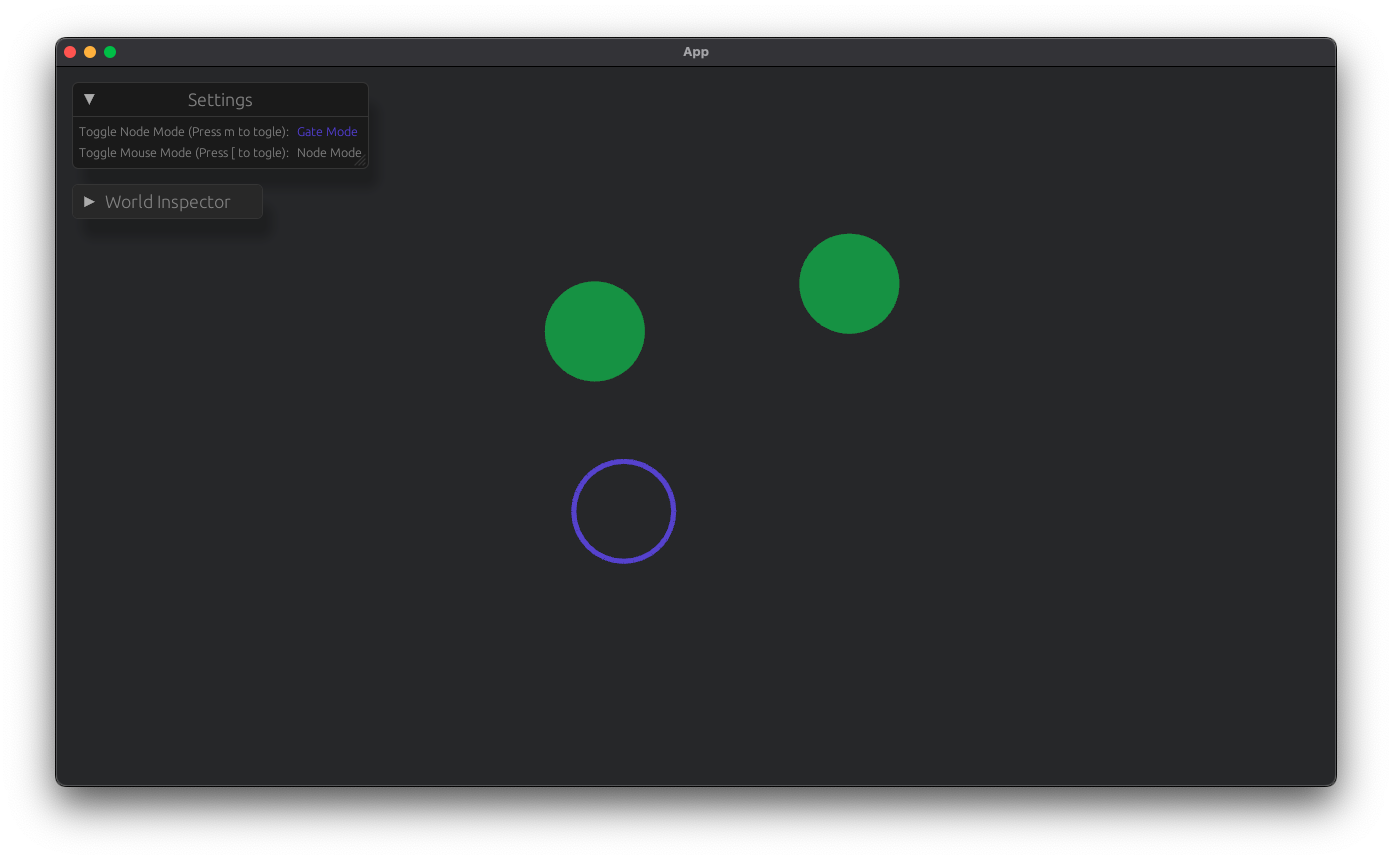
\includegraphics[width=0.3\linewidth]{assets/soft-phase-1-add-node.png}
        \label{fig:soft-phase-1:add-node}
    }
    \subfloat[Add edges]{
        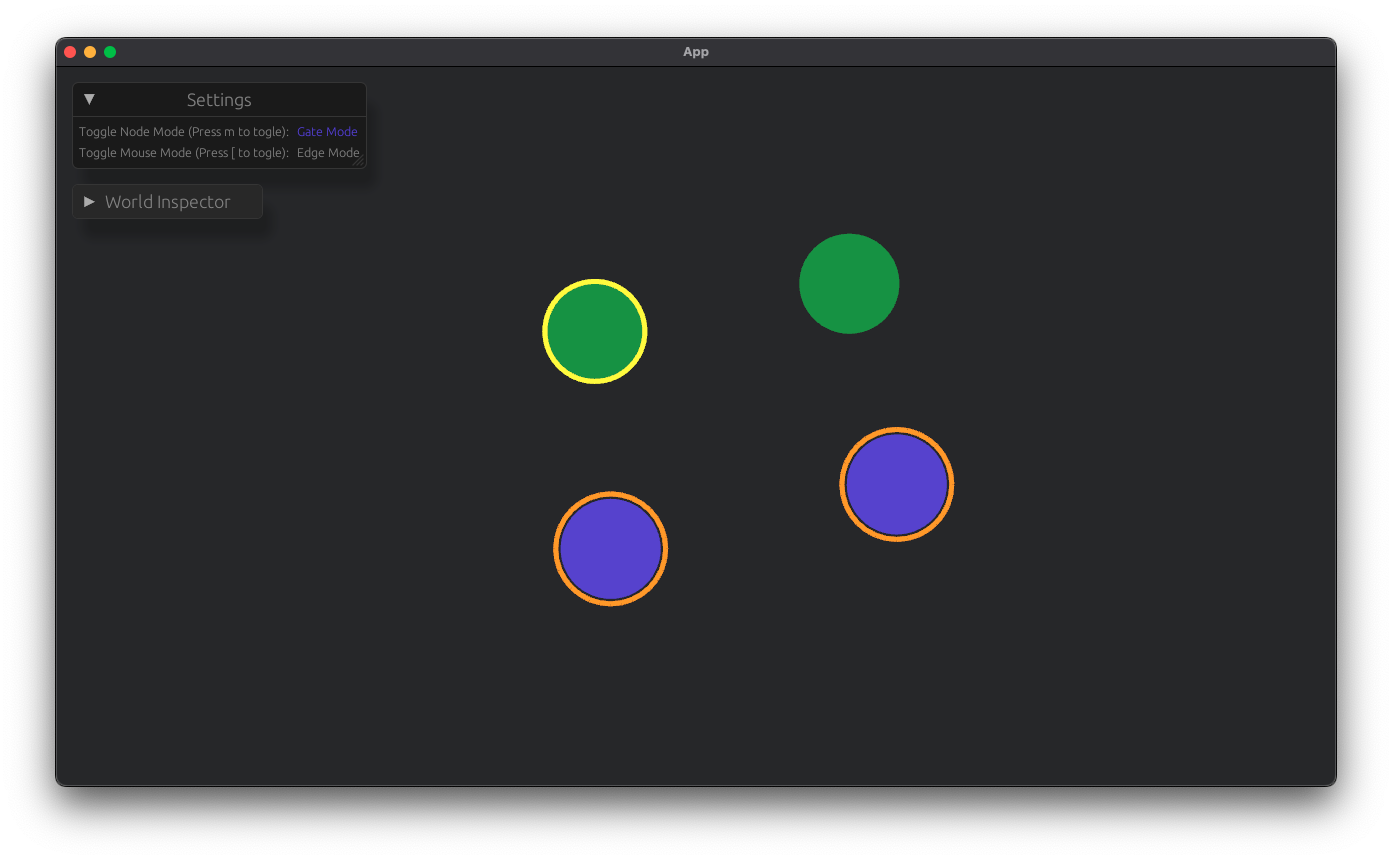
\includegraphics[width=0.3\linewidth]{assets/soft-phase-1-add-edge.png}
        \label{fig:soft-phase-1:add-edge}
    }
    \subfloat[Final state]{
        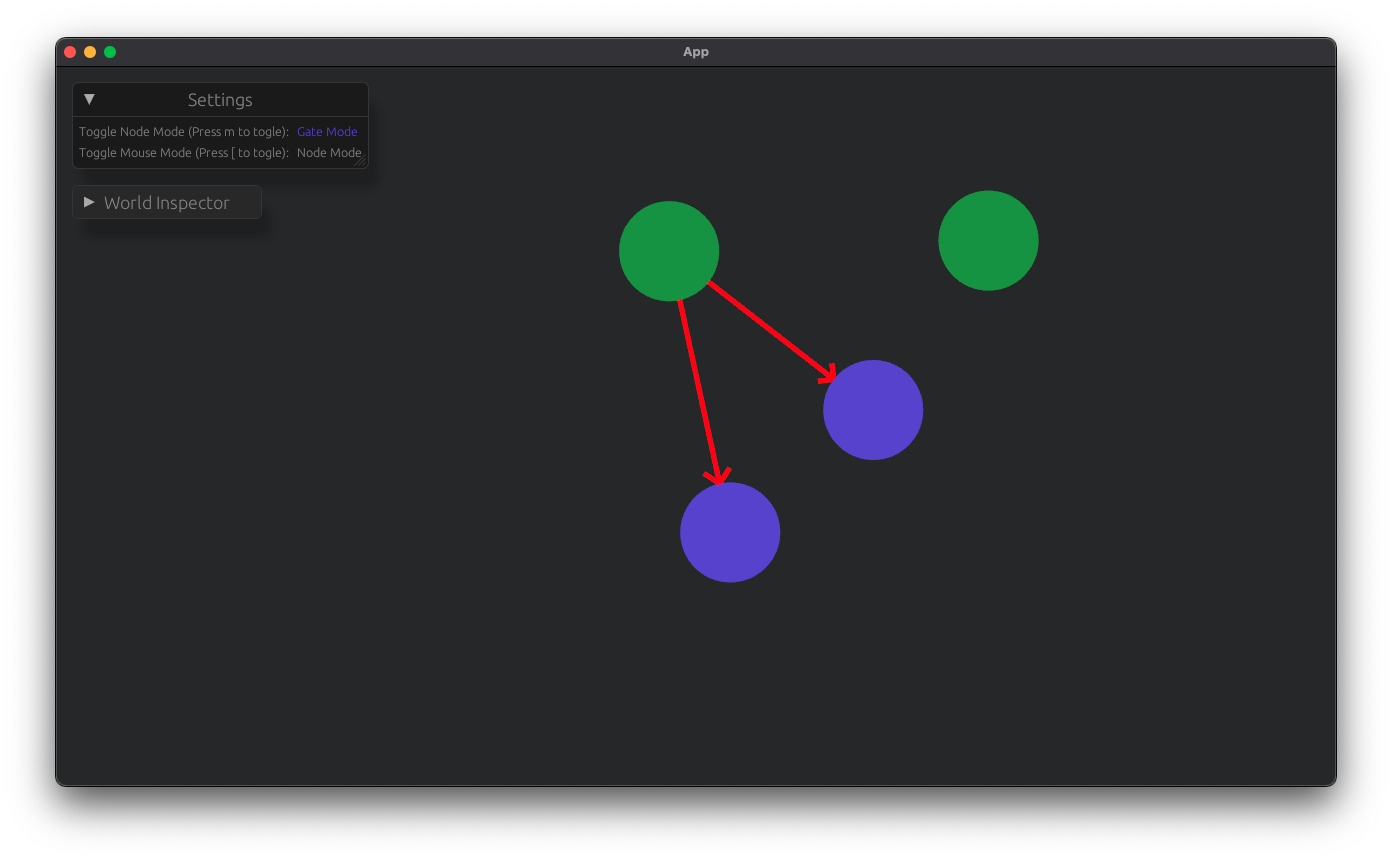
\includegraphics[width=0.3\linewidth]{assets/soft-phase-1-final-state.png}
        \label{fig:soft-phase-1:final-state}
    }
    \caption{Screenshots of different states of the visualisation tool}
    \label{fig:soft:current-phases}
\end{figure}








\section{Research Methodology} 
\subsection{Tools and Resources}

Talk about obsidian:
* Kanban
* Graph view
* Canvas
* Excalidraw
* Zettlekasten system

Github:
* Progress management



\subsection{Timeline and Next Steps}

Add missing gantt chart


\subsubsection{Theory Crafting Next steps}

Our next steps will focus mainly on two directions. One is lowering the bound as we declare in our conjecture with the
usage of snake embeddings. We believe that each dimension can be parsimoniously reduced with another. This implies
that, if we can show that $\forall n \in \mathbb{N}_{\geq 3}: \textsc{\#nD-StrongSperner} \subseteq \textsc{\#2D-StrongSperner}$
we get to prove our conjecture.


With regards to, our second direction, we want to emphasize on the hardness of \textsc{PureCircuit}.
Or more specifically we will investigate as to if any of the following statements hold true.

\begin{gather*}
    \exists n, \alpha \in \mathbb{N}_{\geq 2}:
    \textsc{\#SourceOrExcess}(\alpha,1) - 1  \subseteq \textsc{\#nD-StrongSperner} -1 \\
    \exists n \in \mathbb{N}_{\geq 2}: \textsc{\#SourceOrExcess}(n,1) - 1 \subseteq \textsc{\#PureCircuit} -1 \\
\end{gather*}

We believe the above two should be our next steps in order to get close to the main question of our project.
Ideally generalising, the above reductions to the infinity hierarchy of
$\textsc{\#SourceOrExcess}(\cdot,1)$ would be ideal as it may lead to finding an overall upper bound
towards the entire $\textsc{\#PPAD} -1$ class.


\subsubsection{Software Next Steps}

In the next steps we aim to complete the tasks that were mentioned in the above table,
as well as finding a solution or even better finding all possible solutions. Of
course due to the nature of the problem, finding a single or all solutions for big instances
is computationally difficult. We aim to investigate a method introduced by Eichelberger, where
he utilised repeated applications of the circuit to detect oscillations and replace them with
$\bot$ values. The usage of that procedure was to detect hazard but aim to utilise that procedure
as a heuresaaaawtical approach to reach a satisfying assignment. We do not primarily aim
to fully optimise these algorithms, as the project focuses more on analysing the theoritical findings
of \textsc{PureCircuit}.



Altrenatively, one can use some facts of \textsc{PureCircuit} showed by Deligkas et al.
\cite{deligkasPureCircuitTightInapproximability2024}, were under specific 
gate sets, one can find a \textsc{PureCircuit} instance in polynomial time.
Additionally we were able to find instances or variants of \textsc{PureCircuit}
that are much easier. Conditions like acyclicity make our problem much easier to deal with
or permutation free circuit, make the problem easier to solve.
But just because a solution can be easy to find, does not imply that finding the total number of solutions
is easy, as \cite{valiantComplexityComputingPermanent1979} indicated, or from a more direct
example by \cite{aroraComputationalComplexityModern2009}, where
$$
\textsc{HamiltonianCycle} \leq \textsc{\#Cycle}
$$




%% TODO add  gantt chart
\subsection{Appraisals and Reflections}

\subsubsection{Reflections}
Over the last couple of months I made a lot of mistakes whilst working with the project.
Was just not focusing enough or spending enough time to do the necessary research needed
to comprehend the topic. Moreover, I spent time focusing on the wrong aspects of my assingment.
An example of that is referred to the sections were we showed variants of our pure circuit
that have a combinatorial interpretation. Although in a way one can argue that we indeed 
demonstarted aspects of our problem that are easy, the main focus comes when trying 

\subsubsection{Lessons Learned}


\section{Project Plan} 
\input{sections/project_plan}

\section{Conclusion} 
\lipsum[1]


    
\bibliographystyle{IEEEtran}
\bibliography{dissertation}

\end{document}
